\documentclass{beamer}

\usepackage[utf8]{inputenc}
\usepackage{adjustbox}
\usepackage[T2A]{fontenc}
\usepackage{amssymb}
\usepackage{amsmath}
\usepackage{mathrsfs}
\usepackage{euscript}
\usepackage{upgreek}
\usepackage[english,russian]{babel}
\usepackage{array}
\usepackage{theorem}
\usepackage[all]{xy}
\usepackage{subfig}
\usepackage{epstopdf}   
\usepackage{tikz}       
\usepackage{pgfplots}   
\usepackage{color}
\usepackage{ifthen}
\usepackage{url}
\usepackage{makeidx}
\usepackage{pb-diagram}
\usepackage{balance}
\usepackage{multirow} 
\usepackage{bibentry}
\usepackage{booktabs}
\usepackage{cmap}
\usepackage{amsthm}
\usepackage[linesnumbered,ruled,vlined]{algorithm2e}
\usepackage[absolute]{textpos}
\usepackage{fleqn,psfrag,wrapfig,tikz}
\usepackage{algpseudocode}
\usepackage{amsmath}

\DeclareMathOperator*{\argmin}{arg\,min}
\DeclareMathOperator*{\argmax}{arg\,max}

\usepackage{graphics}
\usepackage{graphicx} % Allows including images
\usepackage{tabularx}

%\graphicspath{ {/home/study/4course/2019-Project-44/data/pics/} }

%\usepackage{jmlda}
\usetheme{Warsaw}
\usecolortheme{sidebartab}
%\definecolor{beamer@blendedblue}{RGB}{15,80,120}
%----------------------------------------------------------------------------------------------------------
\title[\hbox to 56mm{Project 1  \hfill\insertframenumber\,/\,\inserttotalframenumber}]
{Network Science. Project 1}
\author[В.\,С.~Бучнев]{Валентин Бучнев}
\institute[МФТИ]{Московский физико-технический институт \\
    Физтех-школа прикладной математики и информатики
    \vspace{0.3cm} \\
}

\date{
    Москва,\\
    2020\,г.
}

\begin{document}
\captionsetup[figure]{labelformat=empty}

\begin{frame}
\titlepage % Print the title page as the first slide
\end{frame}

\begin{frame} {Описание графа друзей}
\begin{figure}[h!t]\center
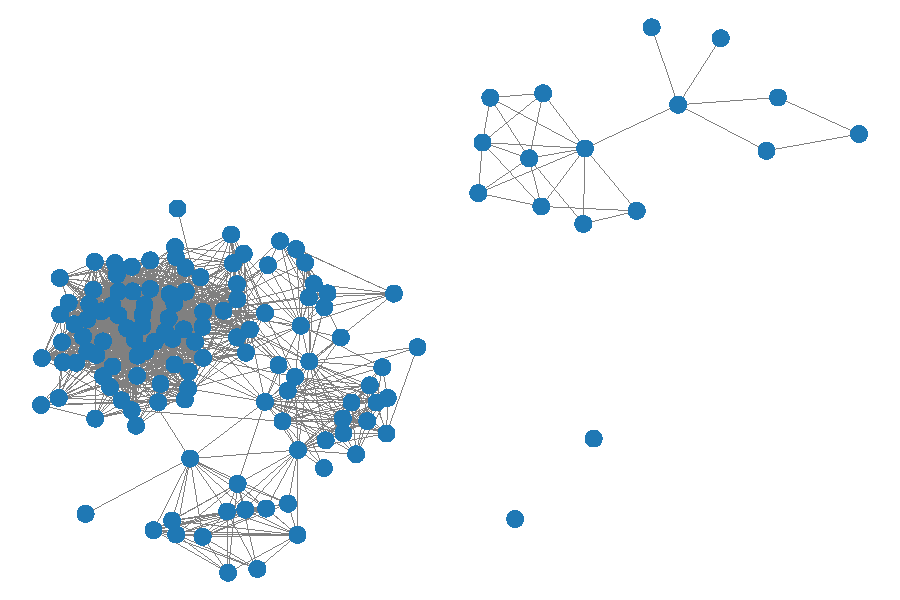
\includegraphics[width=1\textwidth]{graph.pdf}
\label{fig1}
\end{figure}
\end{frame}

\begin{frame} {Описание графа друзей}
\begin{block} {Свойства}
\begin{itemize}
	\item Вершин: 138
	\item Ребер: 1556
	\item Диаметр: 5
	\item Коэффициент кластеризации: 0.62
\end{itemize}
\end{block}

\begin{block} {Аттрибуты вершин}
\begin{itemize}
	\item Город
	\item Университет
\end{itemize}
\end{block}

\end{frame}

\begin{frame} {Описание графа друзей}
\begin{figure}[h!t]\center
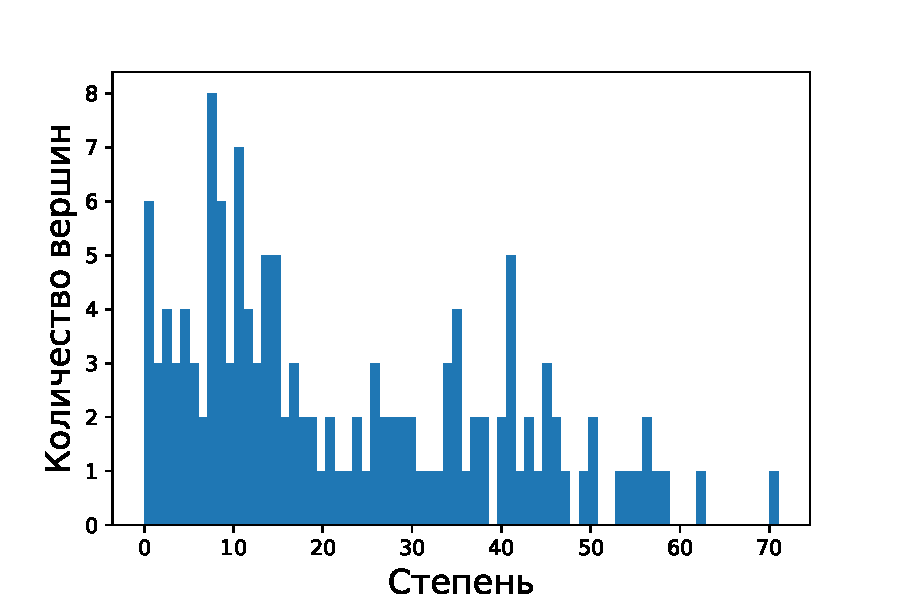
\includegraphics[width=1\textwidth]{degree.pdf}
\label{fig2}
\end{figure}
\end{frame}

\begin{frame} {Degree centralities}
\begin{figure}[h!t]\center
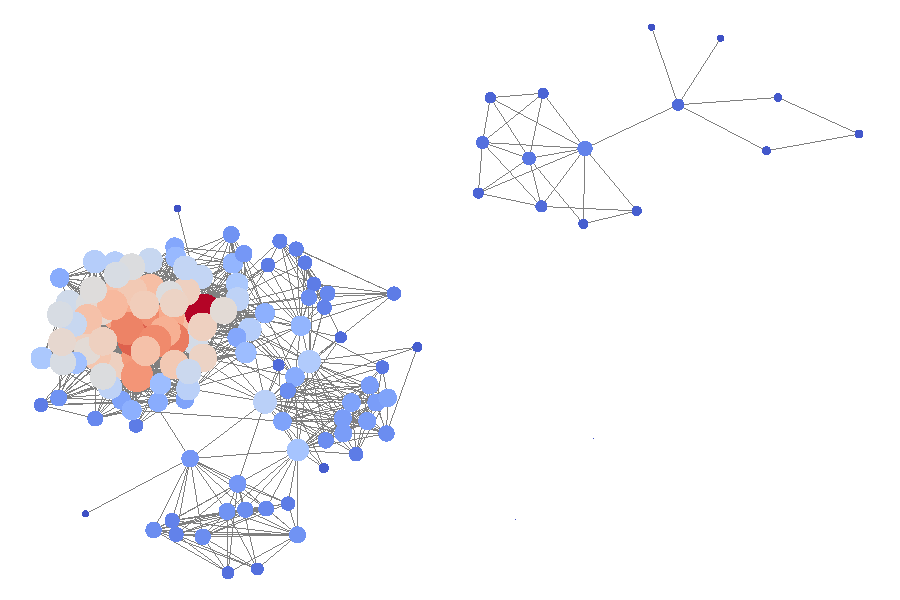
\includegraphics[width=1\textwidth]{degree_centralities.pdf}
\label{fig3}
\end{figure}
\end{frame}

\begin{frame} {Closeness centralities}
\begin{figure}[h!t]\center
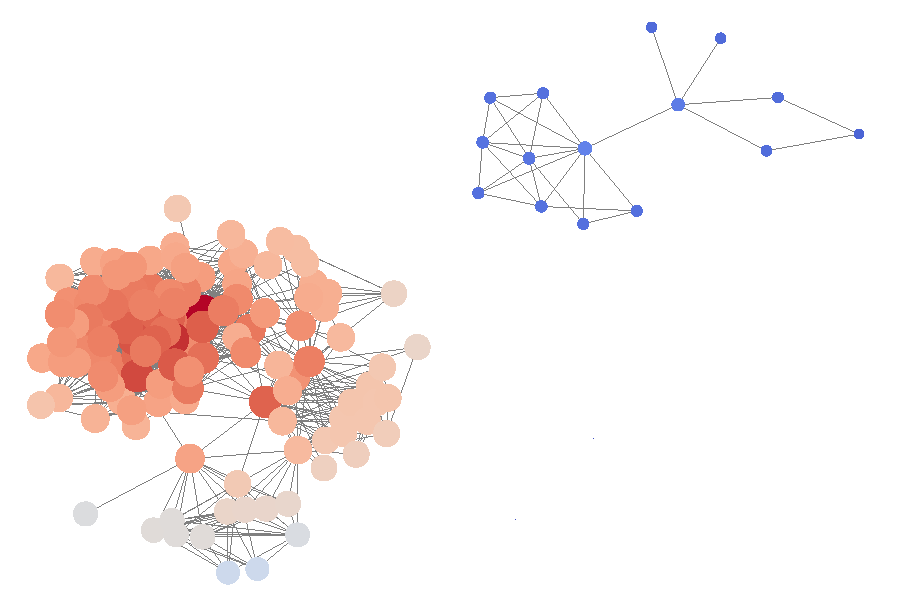
\includegraphics[width=1\textwidth]{closeness_centralities.pdf}
\label{fig4}
\end{figure}
\end{frame}

\begin{frame} {Betweenness centralities}
\begin{figure}[h!t]\center
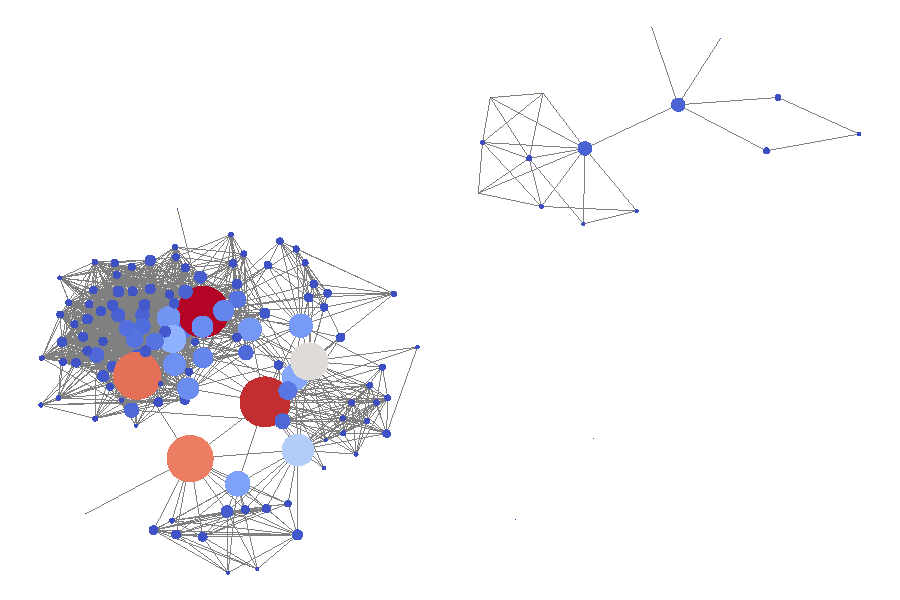
\includegraphics[width=1\textwidth]{betweenness_centralities.pdf}
\label{fig5}
\end{figure}
\end{frame}

\begin{frame} {Pagerank}
\begin{figure}[h!t]\center
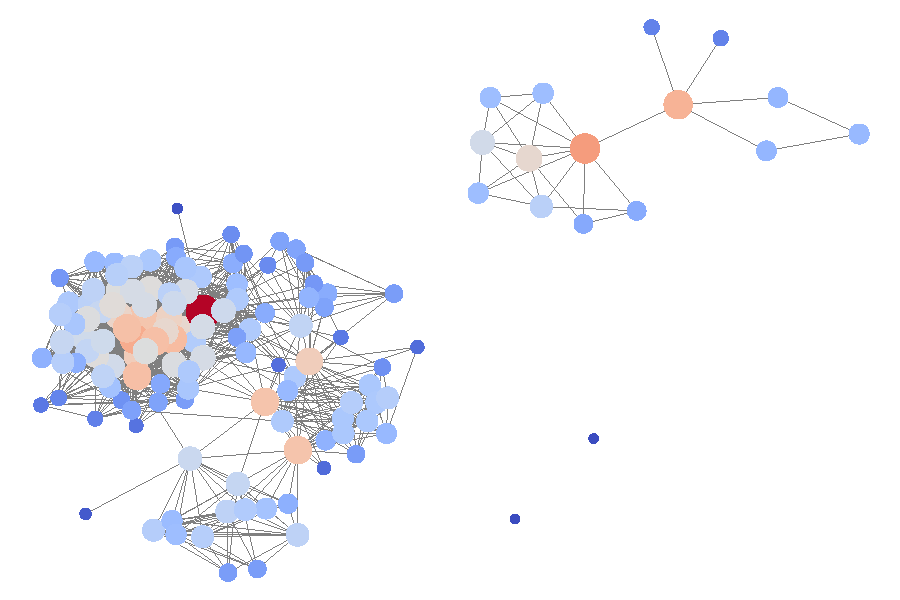
\includegraphics[width=1\textwidth]{pagerank.pdf}
\label{fig6}
\end{figure}
\end{frame}

\begin{frame} {Assortative mixing}
\begin{figure}[h!t]\center
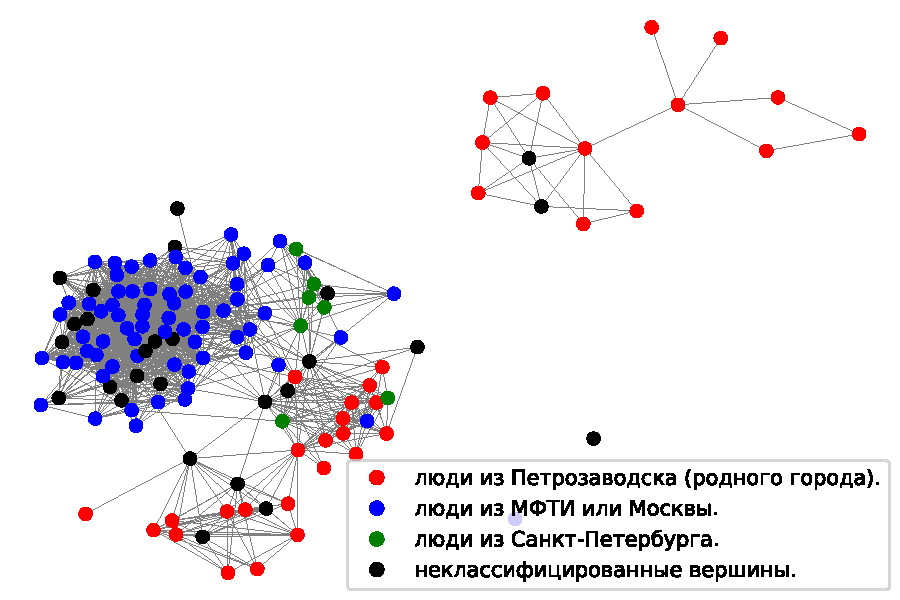
\includegraphics[width=1\textwidth]{assortative_mixing.pdf}
\label{fig7}
\end{figure}
\end{frame}


\begin{frame} {Node structural similarity}
\begin{figure}[h!t]\center
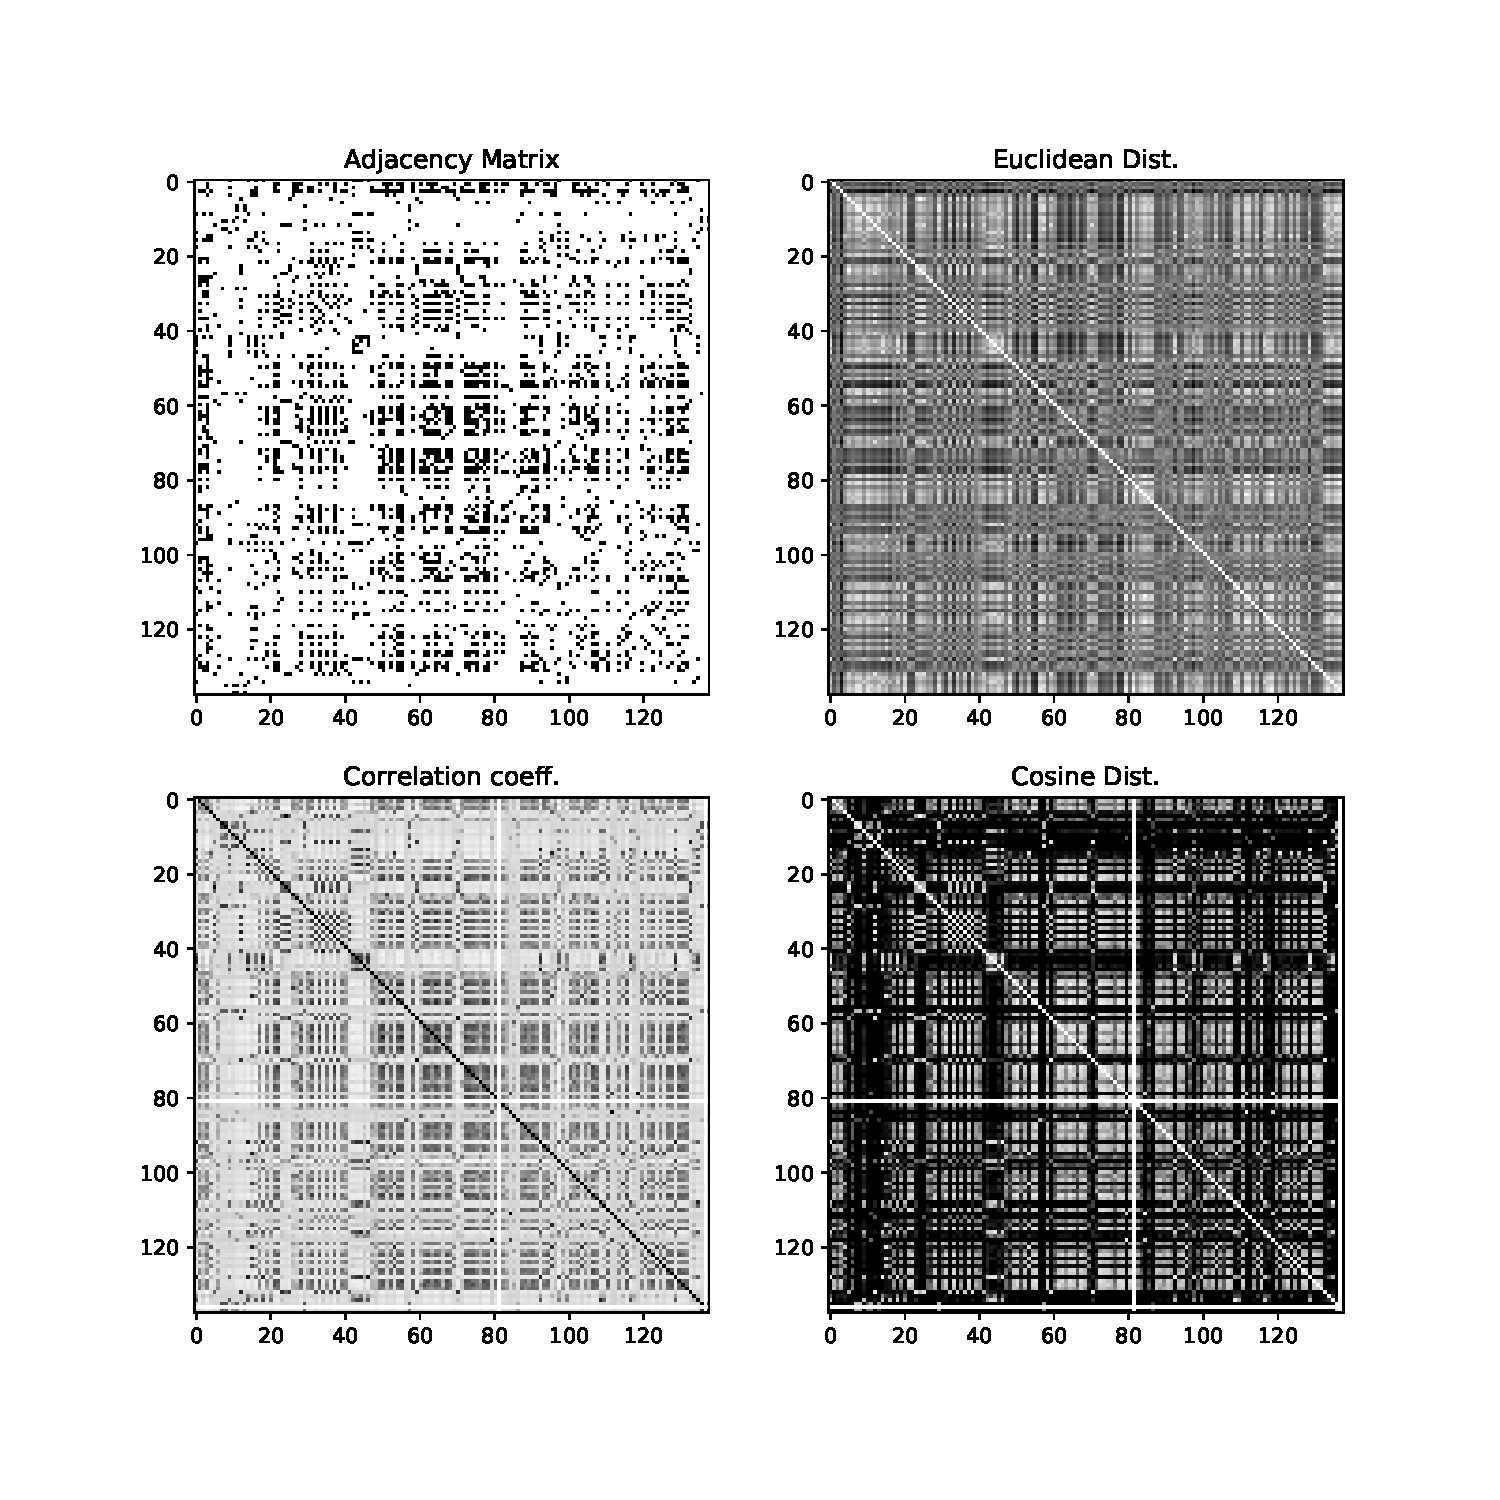
\includegraphics[width=0.8\textwidth]{similarity.pdf}
\label{fig8}
\end{figure}
\end{frame}

\begin{frame} {The closest random graph model}

\begin{block}{}
Рассмотрим распределение степени вершины при разных моделях.
\end{block}

\begin{table}[h]
\begin{center}
\label{table1}
\begin{tabularx}{\textwidth}{|c|>{\centering\arraybackslash}X|>{\centering\arraybackslash}X|>{\centering\arraybackslash}X|>{\centering\arraybackslash}X|>{\centering\arraybackslash}X|}
\hline
	\centering model  & degree distribution & loglikelihood\\
	\hline
	Erdos-Renyi uniform model & $Bin(n-1, 0.5)$ & -6004.14\\
	\hline
	Erdos-Renyi binomial model & $Pois(22.57)$ & -1195.32\\
	\hline
	Preferential attachment model & $Power(-3)$ & -1155.82\\
\hline
\end{tabularx}
\end{center}
\end{table}

\end{frame}

\begin{frame} {Clique search}
\begin{figure}[h!t]\center
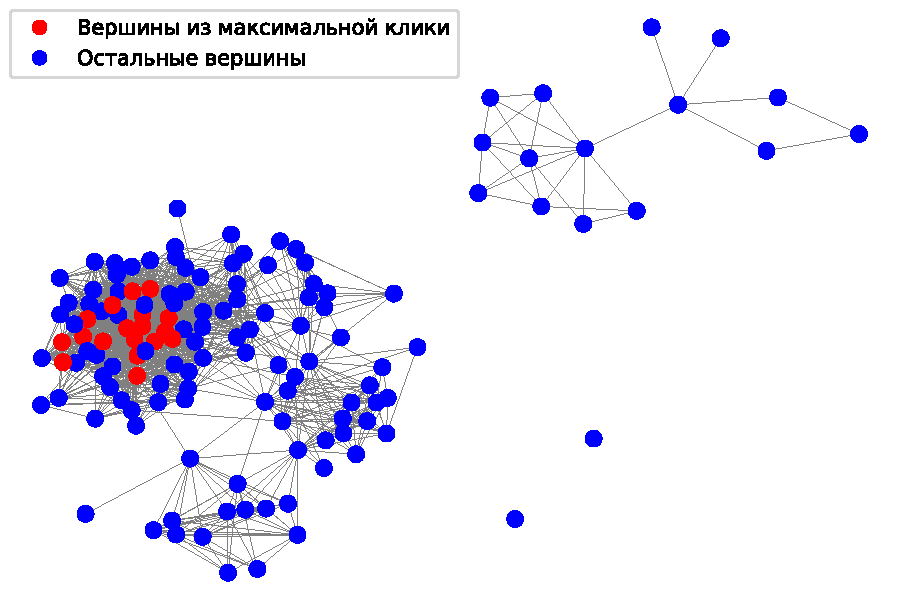
\includegraphics[width=1\textwidth]{clique.pdf}
\label{fig9}
\end{figure}
\end{frame}

\begin{frame} {Community detection (Markov Clustering Algorithm)}
\begin{figure}[h!t]\center
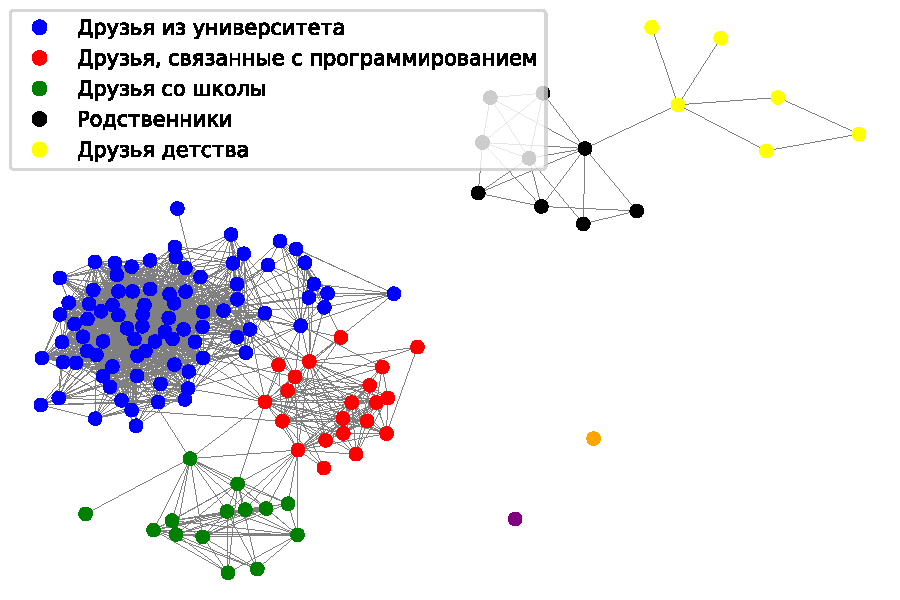
\includegraphics[width=1\textwidth]{clusters.pdf}
\label{fig9}
\end{figure}
\end{frame}


\end{document}